\documentclass{article}
\usepackage{longtable}
\usepackage{makecell}
\usepackage{float}
\usepackage{graphicx}
\usepackage{bm}
\usepackage{placeins}
\usepackage{threeparttable} 
\usepackage{multirow}
\usepackage{aligned-overset}
\usepackage[slantfont,boldfont]{xeCJK}
\usepackage{fontspec}
\renewcommand{\arraystretch}{1.5}
\setCJKmainfont{SimSun}
\setmainfont{SimSun}
\setsansfont{SimSun}

\title{电位差计实验报告}
\author{2411545 邱凯锐}
\date{2025.3.17}

\begin{document}
\maketitle
\section{实验目的}
\hspace*{2em}1.了解电位差计的电位补偿原理和结构。\\
\hspace*{2em}2.掌握电位差计的校准方法和测量方法。\\
\hspace*{2em}3.测量待测电源分别位于0.1档、0.6档和1.2档时未知电动势$E_X$的大小,电位差计灵敏度,并计算不确定度$u$。
\section{实验原理}

\subsection{电位差计原理——电压补偿原理}
\hspace*{2em}Figure 1是将被测电动势的电源\(E_x\)与一已知电动势的电源\(E_0\)“\(+\)”端对“\(+\)”端,“\(-\)”端对“\(-\)”端地联成一回路,在电路中串联检流计“\(G\)”,若两电源电动势不相等,即\(E_x\neq E_0\),回路中必有电流,检流计指针偏转;如果电动势\(E_0\)可调并已知,那么改变\(E_0\)的大小,使电路满足\(E_x = E_0\),则回路中没有电流,检流计指示为零,这时待测电动势\(E_x\)得到已知电动势\(E_0\)的完全补偿。可以根据已知电动势值\(E_0\)定出\(E_x\),这种方法叫补偿法。如果要测任一电路中两点之间的电压,只需将待测电压两端点接入 。\\
\hspace*{2em}上述补偿回路代替 \(E_x\),根据补偿原理就可以测出它的大小。我们知道,用电压表测量电压时,总要从被测电路上分出一部分电流,从而改变了被测电路的状态,用补偿法测电压时,补偿电路中没有电流,所以不影响被测电路的状态。这是补偿测量法最大的优点和特点。
\begin{figure}[ht]
    \centering
    \begin{minipage}{0.45\textwidth} % 调整宽度为总宽度的45%
        \centering
        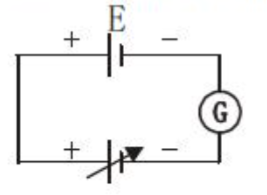
\includegraphics[width=3cm]{2.1.png} % 替换为你的图片路径
        \caption{电压补偿法}
    \end{minipage}\hfill
    \begin{minipage}{0.45\textwidth}
        \centering
        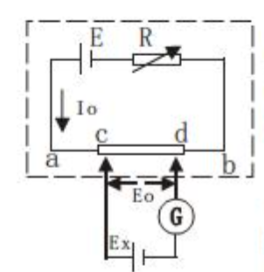
\includegraphics[width=3cm]{2.2.png} % 替换为你的图片路径
        \caption{电位差计}
    \end{minipage}
\end{figure}\\
\hspace*{2em}按电压补偿原理构成的测量电动势的仪器称为电位差计。由上述补偿原理可知,采用补偿法测量电动势对 \(E_O\) 应有两点要求:(1)可调。能使 \(E_O\) 和 \(E_X\) 补偿。(2)精确。能方便而准确地读出补偿电压 \(E_O\) 大小,数值要稳定。
是实现补偿法测电动势的原理线路,即电位差计的原理图。采用精密电阻 \(R_{ab}\) 组成分压器,再用电压稳定的电源 \(E\) 和限流电阻 \(R\) 串联后向它供电。只要 \(R_{cd}\) 和 \(I_O\) 数值精确,则图中虚线内 \(cd\) 之间的电压即为精确的可调补偿电压 \(E_O\),\(E_O\) 和 \(E_X\) 组成的回路 \(cdGE_X\) 称为补偿回路。

\subsection{电位差计的校准}
\hspace*{2em}要想使回路的工作电流等于设计时规定的标准值 \(I_O\),必须对电位差计进行校准。方法如图4所示。\(E_S\) 是已知的标准电动势,根据它的大小,取 \(cd\) 间电阻为 \(R_{cd}\),使 \(R_{cd} = E_S/I_O\),将开关 \(K\) 倒向 \(E_S\),调节 \(R\) 使检流计指针无偏转,电路达到补偿,这时 \(I_O\) 满足关系 \(I_O = E_S/R_{cd}\),由于已知的 \(E_S\)、\(R_{cd}\) 都相当准确,所以 \(I_O\) 就被精确地校准到标准值,要注意测量时 \(R\) 不可再调,否则工作电流不再等于 \(I_O\)。\\
\begin{figure}[ht]
    \centering
    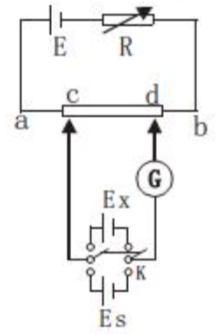
\includegraphics[width=4cm]{2.3.png} % 替换为你的图片路径
    \caption{电位差计的校准}
\end{figure}\\

\section{实验设备}
\textbf{87-1型学生式电位差计(杭州大华)}\\
\hspace*{1em}1.电位差计基本误差为\(\pm0.2\%\)(以满度值计算);电位差计的工作电流为\(5.5\)毫安。\\
\hspace*{1em}2.电位差计有“\(\times1\)”和“\(\times0.1\)”二档倍率:\\
\hspace*{2em}“\(\times1\)”档的测量上限为\(1.710\)伏,最小分度为\(0.0001\)伏;\\
\hspace*{2em}“\(\times0.1\)”档的测量上限为\(171.0\)毫伏,最小分度为\(0.01\)毫伏。\\
\hspace*{1em}3、本电位差计的工作电源为\(2.8\sim3.2\)伏,电源回路的工作电流调节可采用“内接\(R\)”。\\
\hspace*{1em}4、标准电势\(1.01860\)伏,被测电势\(0 - 1900\mathrm{mV}\)分\(11\)挡。
\begin{figure}[h]
    \centering
    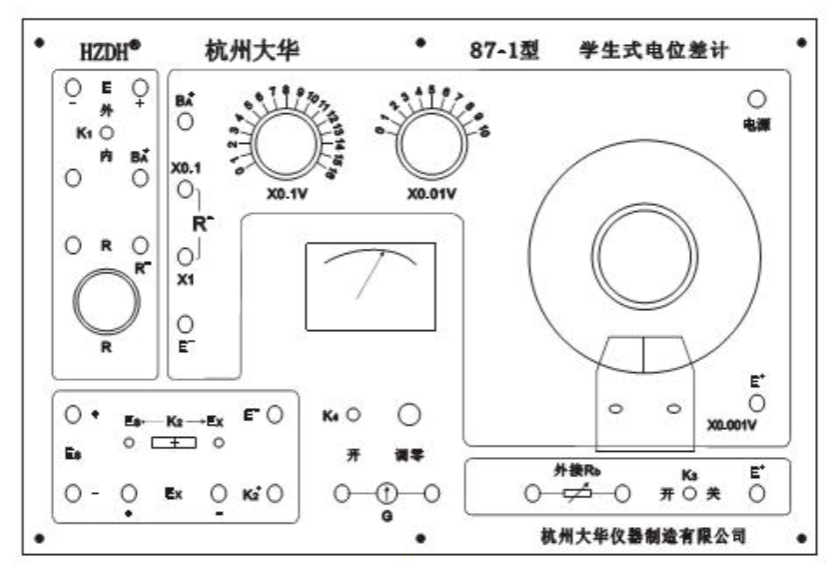
\includegraphics[width=9cm]{3.1.png} % 替换为你的图片路径
    \caption{电位差计}
\end{figure}
\begin{figure}[h]
    \centering
    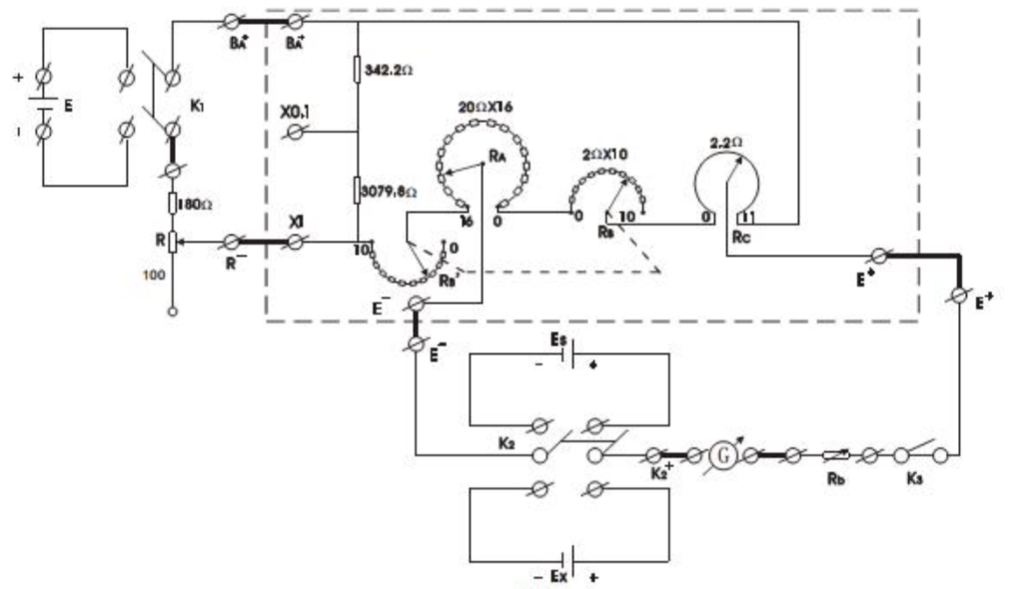
\includegraphics[width=9cm]{3.2.png} % 替换为你的图片路径
    \caption{电位差计内部电路}
\end{figure}

\section{实验内容}

1.\textbf{按照电路图连接电路}\\
2.\textbf{校准学生式电位差计}\\
\hspace*{2em}使用电位差计之前,先要进行校准,使电流达到规定值。先放好 \(R_A\)、\(R_B\) 和 \(R_C\),使其电压刻度等于标准电池电动势。合上 \(K_1\)、\(K_3\),将 \(K_2\) 推向 \(E_S\)(间歇使用),并同时调节 \(R\),使检流计无偏转(指零),为了增加检流计灵敏度,应逐步减少 \(R_b\),如此反复开、合 \(K_2\) ,确认检流计中无电流流过时,则 \(I_O\) 已达到规定值。\\
3.\textbf{测量未知电池电动势$E_X$}\\
\hspace*{2em}按待测电动势的近似值放好 \(R_A\)、\(R_B\)、\(R_C\),\(K_2\) 推向 \(E_X\) 并同时调电位差计 \(R_A\)、\(R_B\)、\(R_C\)使检流计无偏转(在测 \(E_X\) 的步骤中 \(R\) 不能变动),此时 \(R_A\)、\(R_B\) 和 \(R_C\) 显示的读数值即为 \(E_X\) 值。
\\
\hspace*{2em}重复“校准”与“测量”两个步骤。共对 \(E_X\) 测量5次,取 \(E_X\) 的平均值作为测量结果。\\
4.\textbf{电位差计的灵敏度}\\
\hspace*{2em}当电位差计测量达到平衡时,检流计的指针不再偏转,但这并不能说明测量回路中的电流绝对为零,这反映了电位差计对平衡的判别能力。为此引入电位差计电压灵敏度的概念,定义为:
$$
S=\frac{\Delta n}{\Delta U}(格/\mathbf{V})
$$
式中\(\Delta U\)为电位差计平衡后,使分度电阻\(R\)上\(A\)、\(C\)间电压调离平衡时的电压改变值,\(\Delta n\)为此时检流计\(G\)偏转的格数。
\\
\\
\hspace*{2em}分别测量待测电势\(0.1\)档、\(0.6\)档和\(1.2\)档的电势输出,重复测量5次取平均,并测量电位差计灵敏度。
\section{实验数据}
\subsection{不确定度u计算方法}
\hspace*{2em}A类不确定度:
$$
u_a=1.14\sqrt{\frac{\sum_{i=1}^{n}(E_{x_i}-\overline{E_x})^2}{n(n-1)}}
$$
\hspace*{2em}B类不确定度:
$$
u_{b_1}=\frac{\Delta_{仪}}{\sqrt{3}}
$$
$$
u_{b_2}=\frac{\delta}{ \overline{S} }
$$
\hspace*{2em}其中$\Delta_{仪}=2\times 10^{-5}\mathbf{V}(\times 1档)$,$\Delta_{仪}=2\times 10^{-6}\mathbf{V}(\times 0.1档)$,$\delta=0.2$。
$$
u=\sqrt{{u_a}^2+{u_{b_1}}^2+{u_{b_2}}^2}
$$

\subsection{实验数据}
以下数据中$\Delta n=5$\\
1.\textbf{电势0.1档}
\begin{longtable}{ccccc}
    %\centering
    \label{table:longtable_example} \\
    % 下面是表头
    \hline  组别 & $E_x(\mathbf{V})$ & $E_{x}'(\mathbf{V})$ & $\Delta E$ & S \\ \hline 
    \endfirsthead
    % 下面数字3的意思是表格的列数
    \multicolumn{5}{c}%
    {{\bfseries continued from previous page}} \\
    \hline  组别 & $E_x(\mathbf{V})$ & $E_{x}'(\mathbf{V})$ & $\Delta E$ & S \\ \hline 
    % 注意这里把表头复制了一遍,因为在新的页面也会展示一下表头,不然表格不方便阅读
    \endhead
    \hline \multicolumn{5}{r}{{Continued on next page}} \\ \hline
    \endfoot
    \hline \hline
    \endlastfoot
    1 & 0.100103 & 0.100148 & 0.000045 & 111111.1111 \\ \hline
2 & 0.100111 & 0.100150 & 0.000039 & 128205.1282 \\ \hline
3 & 0.100115 & 0.100154 & 0.000039 & 128205.1282 \\ \hline
4 & 0.100110 & 0.100160 & 0.000050 & 100000      \\ \hline
5 & 0.100113 & 0.100158 & 0.000045 & 111111.1111 \\ \hline
\end{longtable}

\begin{longtable}{cccccc}
    %\centering
    \label{table:longtable_example} \\
    % 下面是表头
    \hline  $\overline{E_x}(\mathbf{V})$ & $\overline{S}$ & $u_a$ & $u_{b_1}$ & $u_{b_2}$ & u \\ \hline 
    \endfirsthead
    % 下面数字3的意思是表格的列数
    \multicolumn{6}{c}%
    {{\bfseries continued from previous page}} \\
    \hline  组别 & $E_x(\mathbf{V})$ & $E_{x}'(\mathbf{V})$ & $\Delta E$ & S \\ \hline 
    % 注意这里把表头复制了一遍,因为在新的页面也会展示一下表头,不然表格不方便阅读
    \endhead
    \hline \multicolumn{6}{r}{{Continued on next page}} \\ \hline
    \endfoot
    \hline \hline
    \endlastfoot
    0.100110 & 115726.4957 & 0.000002 & 0.000001 & 0.000002 & 0.000003 \\ \hline
\end{longtable}
得到结果:$E_x=\overline{E_x}\pm u=(0.100110+0.000003)V$\\

2.\textbf{电势0.6档}
\begin{longtable}{ccccc}
    %\centering
    \label{table:longtable_example} \\
    % 下面是表头
    \hline  组别 & $E_x(\mathbf{V})$ & $E_{x}'(\mathbf{V})$ & $\Delta E$ & S \\ \hline 
    \endfirsthead
    % 下面数字3的意思是表格的列数
    \multicolumn{5}{c}%
    {{\bfseries continued from previous page}} \\
    \hline  组别 & $E_x(\mathbf{V})$ & $E_{x}'(\mathbf{V})$ & $\Delta E$ & S \\ \hline 
    % 注意这里把表头复制了一遍,因为在新的页面也会展示一下表头,不然表格不方便阅读
    \endhead
    \hline \multicolumn{5}{r}{{Continued on next page}} \\ \hline
    \endfoot
    \hline \hline
    \endlastfoot
    1 & 0.59940 & 0.59936 & 0.00004 & 125000      \\ \hline
    2 & 0.59958 & 0.59951 & 0.00007 & 71428.57143 \\ \hline
    3 & 0.59952 & 0.59945 & 0.00007 & 71428.57143 \\ \hline
    4 & 0.59944 & 0.59940 & 0.00004 & 125000      \\ \hline
    5 & 0.59940 & 0.59936 & 0.00004 & 125000  \\ \hline
\end{longtable}

\begin{longtable}{cccccc}
    %\centering
    \label{table:longtable_example} \\
    % 下面是表头
    \hline  $\overline{E_x}(\mathbf{V})$ & $\overline{S}$ & $u_a$ & $u_{b_1}$ & $u_{b_2}$ & u \\ \hline 
    \endfirsthead
    % 下面数字3的意思是表格的列数
    \multicolumn{6}{c}%
    {{\bfseries continued from previous page}} \\
    \hline  组别 & $E_x(\mathbf{V})$ & $E_{x}'(\mathbf{V})$ & $\Delta E$ & S \\ \hline 
    % 注意这里把表头复制了一遍,因为在新的页面也会展示一下表头,不然表格不方便阅读
    \endhead
    \hline \multicolumn{6}{r}{{Continued on next page}} \\ \hline
    \endfoot
    \hline \hline
    \endlastfoot
    0.59947 & 103571.4286 & 0.000041 & 0.000012 & 0.000002 & 0.000042\\ \hline
\end{longtable}
得到结果:$E_x=\overline{E_x}\pm u=(0.59947+0.00004)V$\\

3.\textbf{电势1.2档}
\begin{longtable}{ccccc}
    %\centering
    \label{table:longtable_example} \\
    % 下面是表头
    \hline  组别 & $E_x(\mathbf{V})$ & $E_{x}'(\mathbf{V})$ & $\Delta E$ & S \\ \hline 
    \endfirsthead
    % 下面数字3的意思是表格的列数
    \multicolumn{5}{c}%
    {{\bfseries \tablename\ \thetable{} -- continued from previous page}} \\
    \hline  组别 & $E_x(\mathbf{V})$ & $E_{x}'(\mathbf{V})$ & $\Delta E$ & S \\ \hline 
    % 注意这里把表头复制了一遍,因为在新的页面也会展示一下表头,不然表格不方便阅读
    \endhead
    \hline \multicolumn{5}{r}{{Continued on next page}} \\ \hline
    \endfoot
    \hline \hline
    \endlastfoot
    1 & 1.20001 & 1.20007 & 0.00006 & 83333.33333 \\ \hline
2 & 1.20010 & 1.20002 & 0.00008 & 62500       \\ \hline
3 & 1.20005 & 1.20000 & 0.00005 & 100000      \\ \hline
4 & 1.20001 & 1.19994 & 0.00007 & 71428.57143 \\ \hline
5 & 1.20007 & 1.20003 & 0.00004 & 125000      \\ \hline
\end{longtable}

\begin{longtable}{cccccc}
    %\centering
    \label{table:longtable_example} \\
    % 下面是表头
    \hline  $\overline{E_x}(\mathbf{V})$ & $\overline{S}$ & $u_a$ & $u_{b_1}$ & $u_{b_2}$ & u \\ \hline 
    \endfirsthead
    % 下面数字3的意思是表格的列数
    \multicolumn{6}{c}%
    {{\bfseries \tablename\ \thetable{} -- continued from previous page}} \\
    \hline  组别 & $E_x(\mathbf{V})$ & $E_{x}'(\mathbf{V})$ & $\Delta E$ & S \\ \hline 
    % 注意这里把表头复制了一遍,因为在新的页面也会展示一下表头,不然表格不方便阅读
    \endhead
    \hline \multicolumn{6}{r}{{Continued on next page}} \\ \hline
    \endfoot
    \hline \hline
    \endlastfoot
    1.20005 & 88452.38095 & 0.000020 & 0.000012 & 0.000002 & 0.000023 \\ \hline
\end{longtable}
得到结果:$E_x=\overline{E_x}\pm u=(1.20005+0.00002)V$

\section{思考题与总结}
\textbf{思考题:电位差计的测量精度与哪些因素有关?}\\
\hspace*{2em}标准电源$E_s$的精确程度,检流计$G$的灵敏度,工作电压$E$的稳定性,可调电阻$R_A、R_B和R_C$的精确度,人为因素(操作的规范性和速度)。
\\
\\
\hspace*{2em}本次实验通过我们电位差计测量了未知电动势$E_x$,较为成功地掌握了电位差计的原理和使用方法。在实验操作的过程中,操作的顺序、规范性和熟练度都对测量结果有着不小的影响,这对我们日后进行一些测量精度较高的实验提供了一些经验。
\end{document}